%%
%% This is file `mcmthesis-demo.tex',
%% generated with the docstrip utility.
%%
%% The original source files were:
%%
%% mcmthesis.dtx  (with options: `demo')
%%
%% -----------------------------------
%%
%% This is a generated file.
%%
%% Copyright (C)
%%       2010 -- 2015 by Zhaoli Wang
%%       2014 -- 2019 by Liam Huang
%%       2019 -- present by latexstudio.net
%%
%% This work may be distributed and/or modified under the
%% conditions of the LaTeX Project Public License, either version 1.3
%% of this license or (at your option) any later version.
%% The latest version of this license is in
%%   http://www.latex-project.org/lppl.txt
%% and version 1.3 or later is part of all distributions of LaTeX
%% version 2005/12/01 or later.
%%
%% This work has the LPPL maintenance status `maintained'.
%%
%% The Current Maintainer of this work is Liam Huang.
%%
%%
%% This is file `mcmthesis-demo.tex',
%% generated with the docstrip utility.
%%
%% The original source files were:
%%
%% mcmthesis.dtx  (with options: `demo')
%%
%% -----------------------------------
%%
%% This is a generated file.
%%
%% Copyright (C)
%%       2010 -- 2015 by Zhaoli Wang
%%       2014 -- 2019 by Liam Huang
%%       2019 -- present by latexstudio.net
%%
%% This work may be distributed and/or modified under the
%% conditions of the LaTeX Project Public License, either version 1.3
%% of this license or (at your option) any later version.
%% The latest version of this license is in
%%   http://www.latex-project.org/lppl.txt
%% and version 1.3 or later is part of all distributions of LaTeX
%% version 2005/12/01 or later.
%%
%% This work has the LPPL maintenance status `maintained'.
%%
%% The Current Maintainer of this work is Liam Huang.
%%
\documentclass{mcmthesis}
\mcmsetup{CTeX = false,   % 使用 CTeX 套装时,设置为 true
        tcn = 2013573, problem = C,
        sheet = true, titleinsheet = true, keywordsinsheet = true,
        titlepage = false, abstract = true}
\usepackage{newtxtext}%\usepackage{palatino}
\usepackage{lipsum}
\usepackage{caption}
\usepackage{subfigure}
\usepackage{float}
\usepackage{verbatim}
\title{Global Plastic Waste Model based on Linear Programming and Support Vector Regression}
\author{Team 2013573}
\date{\today}
\begin{document}
\begin{abstract}

Plastic waste (PW) has been one of intractable environmental dilemma for modern humankind. In order to mitigate this tough problem, we combine production of plastics and management of plastic waste to establish a model, which can evaluate the impacts of plastic waste and find out an achievable minimal level of plastic production that can be reduced with a time line.  

Firstly, we develop a plastic waste estimate model based on Product Life Cycle (PLC) theory to calculate the maximal levels of single-use or disposable plastic product waste within the environmental capacity in a certain region or country. Then we independently explore the four possible ends of PW and formulate their impacts on environment by several functions. We use linear programming that includes one particular objective function and four constraints. As a result, we can output the maximal amount of plastic products by analyzing the input digits of any region. 

Secondly, to find out to what extent plastic waste can be minimized, we established an model called HSVR which combines happiness-index analysis and SVR method. By analyzing the characteristics of different regions and people’s living standards, we find out the relationship between the amount of plastics produced and people’s happiness index. Based on this, we can analyze how much plastic production we can reduce without significantly reducing happiness.

Thirdly, we follow the previous happiness index to assess how much human life is changed, and apply the Environmental Assessment of Solid Waste Systems and Technologies (EASEWASTE) model to evaluating how the the environment is affected by plastic reduction. Moreover, we take computable general equilibrium (CGE) model to quantify the effects of the target plastic production. Then we normalized the outputs and into non-dimensional indices, and calculate the weight for each indicator above by the analytic hierarchy process (AHP). The total impact for achieving the confined level is a linear combination of the three indices. 

Furthermore, reduction of plastic production will impact countries unequally because of their different development level. We use dual programming to fine the dual model of the linear programming based model we established first. Then shadow prices of every factor formulated by constraints can be calculated, which indicate the significance of each factors. Then we divided them into environmental and governmental factors. Sensitivity analysis is be used to identify which factors that is most sensitive to a particular country, and the equitable reduction of plastic of the country depends on the categories that its sensitive factors belong to. 

Finally, we analyze how to approach the minimum level following the time line by an achievable way. Many unexpected circumstance would definitely appear so we empirically choose most significant possibilities that may delay or accelerate the achievement process. The ultimate result are specified into a memo which will be provided for ICM.

\begin{keywords}
Plastic waste; LCA; SVR; EASEWASTE; AHP
\end{keywords}
\end{abstract}
\maketitle
%% Generate the Table of Contents, if it's needed.
\thispagestyle{empty}
\tableofcontents
\thispagestyle{empty}
\newpage
%\setcounter{page}{1}
%%

%%
\setcounter{page}{1}
\section{Introduction}
\subsection{Background}

For e-commerce platforms such as Amazon, there is no shortage of the customer's ratings and reviews. Ratings are usually expressed in five grades of 1 to 5 stars, while reviews are expressed in text form, giving customers the opportunity to show their feedback. But how to make good use of this huge rating and reviewing data is also a big challenge. Taking good advantage of these data can not only help companies to provide targeted customer service, find potential high sales and low sales goods but also help them adjust operational strategies, or enhance products in a timely manner\cite{zhang2006lord}.

%The management of the plastic waste is one of the most controversial topic in the discussion on integrated municipal solid waste area.

\subsection{Problem statement}

Now, Sunshine Company plans to launch three new products to sell online: microwave, pacifier and hair dryer. The company has obtained historical ratings and comments from customers of these three products. They hope to dig out effective information from reviews and ratings to help companies better formulate sales strategies and enhance the effectiveness of products. They hope that the following problems can be reasonably solved:

\begin{enumerate}
	\item What is the relationship between product star rating, review and help votes? Can we quantify the reviews and explore the mathematical relationship among them?
	\item Based on task1 to address the following specific requests from the Sunshine Company Marketing Director:
	\begin{enumerate}
	\item How to build a model that can integrate ratings and reviews, and help company get effective information and adjust marketing strategies?
	\item How to describe the reputation of the product from the perspective of time, so as to see and predict the change of the product's reputation in the online market?
	\item Based on text evaluation and rating, how to find potential successful or failed products?
	\item Is there a relationship between a specific star rating and the number of reviews? In other words, what kind of ratings attract customers to comment?
	\item Are subject words of a review, such as "happy", "disappointed" related to specific ratings?
	\end{enumerate}
\end{enumerate}

%\subsection{Our work}
%
%Our work can be summarized as follows:
%
%\begin{itemize}
%	\item To get the maximal level of single-use or disposable plastic products, we build PWEM on the basis of LCA, and applied some logical abstractions, physical derivations, and mathematical methods to accomplished the linear programming process, then out put the estimated maximal level of plastic products. 
%	\item We create our HSVR model to define the miximal level with least negative effects on people’s  living standards, based on the fact that people often do not agree to pay too much for environmental protection.
%	\item Using our moedl, we set an achievable target level of plastic usage and apply quite a few known methods to quantify and combine the given factors for assessing the total influence of achieving our goal. 
%	\item We developed our model to measure the influence of various factors to provide realistic solutions for the mentioned euity issue.
%\end{itemize}

%For task 5, TSM is established for predicting the possible timeline and discuss possible relevant circumstances, then write a specific memo for ICM.

\section{Model Analysis}
\subsection{Data analysis based on LDA and Spearman correlation coefficient}
The product data given contains a lot of information, but the deep-seated information information must be processed through information mining so that it can be used for Sunshine Company. 

During the mining process, there must be some invalid data, so we filter it through data cleaning. Secondly, for the non numerical field in the data -- review, we need to make qualitative analysis. After the key words in the reviews are classified by LDA model\cite{blei2003latent}, we can get the quantitative results. 

Thirdly, we make statistics on the comment itself, and get the characteristic information such as sentence number, average sentence length, etc. And finally, we analyze internal relationship between star ratings and helpful ratings and quantified reviews features by Spearman correlation coefficient\cite{myers2004spearman}.

\subsection{Rating-review based reputation model}
\indent We can infer the reputation of a product from its star rating and reviews. The better the reputation of a product, the higher the potential sales volume of the product. 

Here, we can't simply measure the reputation of a product by star rating or evaluation alone, because there are often situations of "five star with negative feedback" or "one star with praise". Therefore, we integrate star ratings and reviews to build a reputation model. By comparing the reputation of products, Sunshine Company can enhance the stock and publicity of products with high reputation.

In similar way, the reputation calculation needs to first carry out LDA processing on the reviews of a product, and then convert them into discrete level values. 

In order to consider the credibility of the reviews, we also consider several fields such as vine, verified\_purchase, helpful\_votes, and total\_votes, which can measure the accuracy of the review, because reviews with product experience are more credible, and reviews of high helpful votes are more referential.

By modeling and calculating the pacifier samples with more than 25 comments from July to August 2015, we find that in July to August, the reputation of sample 'wubbanub soft toy and pacifier' is higher and the sales prospect is the largest; the reputation of 'Philips aventbpa free another pacifier, 3 + months, green, 2 count' is the lowest and the sales prospect is the worst.

\subsection{Relations between time and reputation}
The reputation of products will fluctuate with the change of time, and the latent regulation may have great inspiration for sunshine company. We can use RBF neural network\cite{li2016nonlinear} to fit (reputation time) function. After getting the fitting curve, we can directly observe the change trend of reputation. Take the pacifier for example,

\begin{itemize}
	\item First of all, we select the sample with the most reviews in the pacifier--'philips avent bpa free soothie pacifier, 0-3 months, 2 pack' with 833 reviews
	\item Then we use the reputation transformation model to get the reputation of all samples
	\item Then, taking one day as the unit time, RBF neural network is used to fit the reputation and time
	\item Finally, according to the fitting curve, we find that the reputation of Philips pacifier has a minimum value on May 30, 2015 and a maximum value on May 10, 2015. In the next question, the causes of the maxima and minima are analyzed.
\end{itemize}

\subsection{Indication of potentially successful or failing product}
As mentioned above, reputation will fluctuate with time, so the curve we fit will naturally have inflection point. Therefore, we define that if the curve will usher in a maximum value, the product will become a potential successful product; if the curve will usher in a minimum value, the product will become a potential failure product.

In order to facilitate processing, we only consider a set of maxima and minima of the curve when modeling. We can cluster the stars and reviews near the maxima and minima of the curve to find the topic words and stars with the highest word frequency. When these themes and stars appear, it means that the reputation of the product will probably usher in a turning point.

In our experiment, it is found that when 'baby cant' and 2-3 stars appear, the reputation of the product will decline, so the product will become a potential failure product; when 'baby love' and 4-5 stars appear, the reputation of the product will rise, and the product will become a potential success product.
\section{Assumptions and justifications}
To simplify the problem, we strive for the following assumptions:
\begin{itemize}
	\item Users can't see the rating stars of other users long ago. 
	
	\item Higher product reputation means better sales prospects.
	
	\item Star ratings in a time period satisfies the normal distribution.
	\item The head and body of a review are always consistent.
	\item Poor reviews with high star rating exists.
	\item Positive reviews with low star rating also exist.
	\item Reviews are more valuable than ratings.
	
%	\item \textbf{The mass of annual plastic production equals to that of the annual plastic waste.} On the one hand, every pound of plastic produced will turn into waste. On the other hand, the lifeline of most sorts of plastic is under 20 so that given situation will not change acutely\cite{Geyer}.
%	
%	\item \textbf{Throughout the life cycle of plastic, the impact of plastic on environment in use phase is negligible.} Main environment issues that are related to plastic merely when it is produced or managed\cite{book}.
%	
%	\item \textbf{Aiming to make plastic waste safely be mitigated, any waste should not be landfilled.} While it is extremely hard for plastic to biodegrate in solid, landfills are in great shortage.\cite{book}.
%	
%	\item \textbf{All the plastic waste produced will be managed.} In the long run, the NET plastic waste discarded in natural environment will approach zero by governments and NGOs’ efforts.
%	
%	\item \textbf{The proper quantity of pollutant emission of plastic waste should depend on the contribution of plastic industry to the gross domestic products.} The pollutant emission of plastic waste is just an ordinary part of the total emission, so the responsibility of environmental protection it takes should also be the proportional part, which is roughly estimated by the percentage of GDP that plastic industry contributes.
%	
%	\item \textbf{All the plastic waste is mechanically sorted from plastic waste prior to incineration.} In fact, waste incineration plants are generally very formal and will complete the sorting work. Otherwise, they will be banned soon.
%	
%	\item \textbf{The material recycling facilities(MRFs) that sort and upgrade the received waste stream is the only way to recycled sorted PW.} There is no other mature processing method, and this method is used almost everywhere.
	
\end{itemize}

\section{Parameter Table}

Important symbols that in this article are listed in Table \ref{notation}.
\begin{table}[H] 
	\caption{Notations} 
	\center
	\begin{tabular}{cp{0.7\columnwidth}}
		\toprule 
		Symbols &Definition  \\ 
		\midrule 
		$s_i $& Annual certain plastic production.  \\ 
		$N_i$ & The number of $CO2$ generated by the combustion of 1 molecule specific plastic unit. \\ 
		$EA$ & Emission to air. \\ 
		$EW$ & Emission to water.\\
		$EC$ & Emission of $CO_2$.\\
		$TEA$ & Total emission to air.\\
		$TEW$ & Total emission to water.\\
		$TEC$ & Total emission of $CO_2$.\\
		$CEA$ & Compensatory emission to air of recovery process.\\
		$CEW$ & Compensatory emission to water of recovery process.\\
		$SM$ & Plastic waste into marine.\\
		$M$ & The quantity of annual management of marine plastic.\\
		$V_air$ & Total available air of a specific country/region.\\
		$V_water$ & Total available water of a specific country/region.\\
		$\sigma$ & Proportion of incinerated plastic waste.\\
		$\mu$ & Compensate.\\
		$\theta$ & The percentage of GDP plastic industry contributes, quantified by coefficient.\\
		$\iota$ & Tossil fuel consumption percentage. Generally, $\iota$ equals 4\%.\\
		$k$ & Proportional coefficient of carbon emission per unit of
energy consumption\\
		\bottomrule 
		\label{notation}
	\end{tabular} 
\end{table}

\section{Model Construction}
\subsection{Data analysis model based on LDA and Spearman correlation coefficient}
\subsubsection{Data analysis model based on LDA}
The product data contains thousands of items, so mining the connotation information is very helpful for Sunshine Company.

First of all, we clean the data: remove the data that contains empty fields, random codes and other invalid fields. 

Then we use Latent Dirichlet Allocation(LDA)\cite{blei2003latent} to do analysis, because LDA can identify the hidden subject information in large-scale document collection in an unsupervised way. What's more, it can transform each document sample into a word frequency vector about the topic, thus transforming the text information into intuitive numerical information. Our LDA topic classification modeling is as follows:
\begin{enumerate}
	\item Do text preprocessing on reviews.
		\begin{enumerate}
			\item Unify case and remove symbols and numbers from review text
			\item Delete manually filtered stop words and calibrate misspelled words.
			\item Do word normalization based on stem extraction.
		\end{enumerate}
	\item The key words are extracted and selected by counting the frequency distribution of every word, and then integrated with the high frequency key words selected by the 2-gram model\cite{zhang2006lord}, so that each review is transformed into a key words array.
	\item Put the reviews data into LDA model in the form of  keyword array, and set the number of different topics, then train.
	\item According to coherence score, the number of topics $T_{n}$ that are most suitable is filtered, and the topics are assigned according to the usefulness of keywords in each topic.
	\item Each review is converted into topic frequency vector $R_{vec}=[R_{t\_1},...,R_{t\_n}]$  (where $R_{t\_i}$ is the keyword frequency score under the $i$th topic) according to its keyword array. And take the topic score of the maximum word frequency as the review score (marked as $R_{\beta}$).
\end{enumerate}
The results of LDA subject classification are as follows (take microwave oven as an example):\\
\begin{figure}[H] %H为当前位置,!htb为忽略美学标准,htbp为浮动图形
	\centering %图片居中
	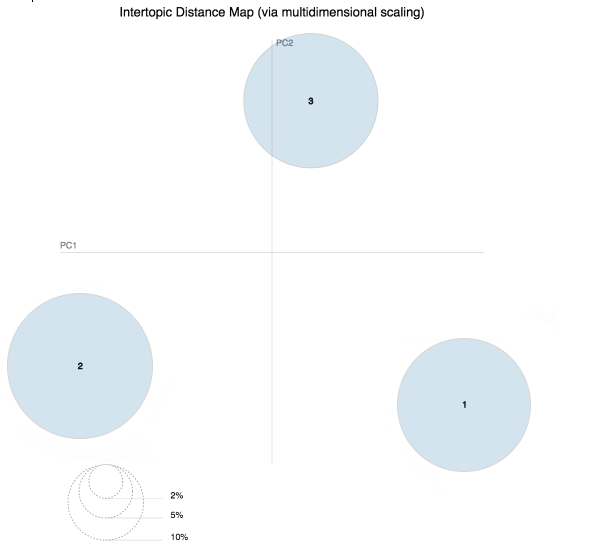
\includegraphics[width=0.5\textwidth]{figures/topic_distribution.png} %插入图片,[]中设置图片大小,{}中是图片文件名
	\caption{The Distribution of Three Topics with Coherence Score 0.543} %最终文档中希望显示的图片标题
	\label{fig4} %用于文内引用的标签
\end{figure}
\begin{figure}[H]
	\centering  %图片全局居中
	\subfigure[topic 1]{
	\label{Fig.sub.sky21}
	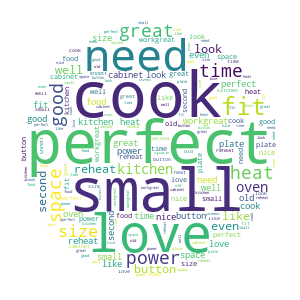
\includegraphics[width=0.3\textwidth]{figures/topic3.png}}
	\subfigure[topic 2]{
	\label{Fig.sub.sky22}
	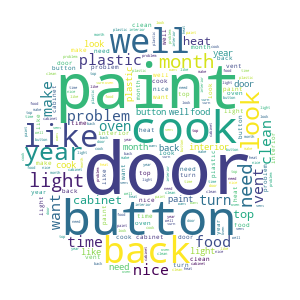
\includegraphics[width=0.3\textwidth]{figures/topic2.png}}
	\subfigure[topic 3]{
	\label{Fig.sub.sky22}
	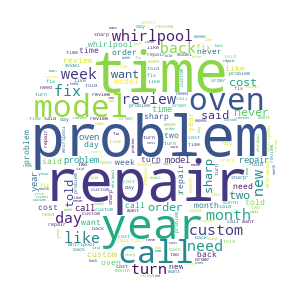
\includegraphics[width=0.3\textwidth]{figures/topic1.png}}
	\caption{Keyword Cloud for Each Topic in Microwave }
	\label{Fig.sky2}
\end{figure}
From the figure, we can see that 
\begin{itemize}
	\item The distance between the three categories is relatively large, and the overall topics consistency score is high. 
	\item According to the key words in the three topics, we can see that topic1 mainly contains a kind of positive emotional key words such as 'perfect', 'nice', 'love' etc;
	\item Topic3 contains some feedback on 'problems' and other specific topics of poor functional evaluation; 
	\item The key words of Topic 2 are relatively neutral, so the three topics are scored 3,2,1 respectively (corresponding to good reviews, medium reviews and poor reviews)
\end{itemize}
And the other two products are also scored in this way which is not show in the paper due to space constraints:
\begin{table}[H]
	\center
	\caption{ Microwave's Topic Score Based on Keyword Attribute}
	\label{type}
	\begin{tabular}{c|c|c}
		\hline
		\textbf{Topic} & \textbf{Key Words} & \textbf{Score} \\ \hline
		TOPIC1                & nice, good, perfect, cook, small, love, need, etc        		&	3          \\ 
		TOPIC2                & paint, door, button, back, light, etc  &	2                 \\ 
		TOPIC3                & repair, problem, return, not work, etc                   		&	1	\\ \hline
	\end{tabular}
\end{table}
\subsubsection{Spearman Correlation Coefficient}
We make characteristic statistics on the reviews, and get the number of sentences in each reviews $R_{s\_{num}}$ and the average length of each sentence $R_{l\_{avg}}$. 

Then we use quantile-based discretization assignment method to grade the continuous value features.

And last, we use spearman correlation coefficient formula as follows to calculate the correlation between the star rate $R {\alpha} $, and the quantitative feature of reviews text ${\{R_{\beta},r_{h},R_{s\_{num}},R_{l\_{avg}},R_{vec}\}}$:
\begin{equation}
	{\frac{\sum_{i}^{n}(a_{i}-\bar{a})(b_{i}-\bar{b})}{{[\sum_{i}^{n}{(a_{i}-\bar{a})}^2\sum_{i}^{n}({b_{i}-\bar{b})}^2]}^{\frac{1}{2}}}}
\end{equation} 

where $a,b$ are two characteristic sequences respectively, ${\bar{a}}$ and ${\bar{b}}$ are the average values of the two sequences respectively.

Taking the microwave oven as an example, the following results are obtained:
\begin{table}[H]
	\center
	\caption{Correlation between Star Rating and Review features}
	\label{type}
	\begin{tabular}{c|c}
		\hline
		\textbf{Feature - Feature} & \textbf{Correlation value} \\ \hline
		star rating$R_{\alpha}$ -  topic score $R_{\beta}$             & 0.651                    \\ 
		star rating$R_{\alpha}$ -  review sentence num  $R_{s\_{num}}$              & 0.209                     \\ 
		star rating$R_{\alpha}$ -  review sentence average length  $R_{l\_{avg}}$              & -0.121                     \\ 
		star rating$R_{\alpha}$ -  review helpful votes  $r_{h}$                & -0.301 	\\ \hline
	\end{tabular}
\end{table}

\begin{table}[H]
	\center
	\caption{Correlation Among Review Features}
	\label{type}
	\begin{tabular}{c|c}
		\hline
		\textbf{Feature - Feature} & \textbf{Correlation value} \\ \hline
		helpful votes$R_{\alpha}$ -   $R_{t\_{mid}}$               & 0.493                     \\ 
		review helpful votes$R_{\alpha}$ -  review sentence average length  $R_{l\_{avg}}$             & 0.459                    \\
		review helpful votes$R_{\alpha}$ -  review sentence num  $R_{s\_{num}}$              & 0.213                     \\ 
		review helpful votes$R_{\alpha}$ -  $R_{t\_{low}}$                & -0.390 	\\ \hline
	\end{tabular}
	\label{table2}
\end{table}
 In table.\ref{table2}, we use $R_{t\_{mid}}$, $R_{t\_{low}}$ to represent the feature: word frequency score of the topic in middle evaluation and in low  evaluation.
 
 From above tables, we can draw the following conclusions:
\begin{enumerate}
	\item The correlation coefficient between star rating and topic score $R_{\alpha}$ is the highest, and it is positive correlation, which shows that some complimentary high-frequency keywords in the positive topic are closely related to the high score ratio of customers. 
	\item Helpful reviews tend to be rated at low and medium star levels.
	\item The highest correlation coefficient between helpful votes and the score of the subject in the middle evaluation indicates that the helpful reviews of these commodities is relatively more pertinent, more objective, and will not praise excessively or turn to the bad side.
	\item The positive correlation between helpful votes and review sentence average length and review sentence number indicates that helpful reviews are relatively long.
	\item According to the above information, Sunshine Company should pay more attention to the longer reviews with medium star rating and more keywords, so as to find out customers' concerns and ideas and improve products.
\end{enumerate}
\subsection{Rating-Review Based Reputation Model}
\label{task_b}
By modeling ratings and reviews, we can get product reputation, and higher reputation means higher potential sales volume, which can help Sunshine Company make better decisions. The modeling process is as follows:

Assume the star rating of the product is $R_{\alpha}$, the review is quantified as $R_{\beta}$, the helpful votes of the review is $R_{h}$, so that unhelpful votes($R_{u}$) is total votes minus helpful votes, net helpful votes is($R_{h}-R_{u}$), We use net helpful votes plus 1 as a factor and multiply the quantified review to judge the credibility of the evaluation.

We use the logarithmic form to make the intermediate calculation smoother, then average the reputation during specific period, and finally refer to the article\cite{subkhankulova2006comparative} we magnified the reputation differences between samples in the form of index, and the reputation model is initially established as follows:

\begin{equation}
	F_{repu} =  e^{\frac{\sum_{i=1}^{n}(log_2(R_{\alpha}+1)+ \beta \times log_2(R_{\beta}\times(R_{h}-R_{u}+1)+1))}{n}}
	\label{priA}
\end{equation}

where n is the number of evaluation in a certain period. For the convenience of processing, when the net helpful votes are negative in the model, it will be set to -1, that is, this kind of comment has no contribution to reputation.

Furthermore, on the one hand, the super parameter $\beta$ should be able to reflect the weight relationship between rating and comment, on the other hand, it should be able to represent the credibility of the review, and the review with the vine or verified\_purchas field equals 'y' is a review that has experienced the product, which is more referential. So the expression of $\beta$ is as follows:

\begin{equation}
	\beta =\left\{\begin{matrix}
1+W_{r} & if &vine &or &verified\_pruchase = 'Y'\\ 
W_{r},& else
\end{matrix}\right.
\label{hyperbeta}
\end{equation}

where $W_{r}$ is the relationship coefficient of rating and review mentioned above. Set 0.61 here.

In order to test our model, we first counted more than 25 pacifier samples from July to August 2015, which are:
\begin{itemize}
	\item 'philips avent bpa free soothie pacifier, 0-3 months, 2 pack, packaging may vary', marked as Sample1
	\item 'wubbanub soft toy and pacifier', marked as Sample2
	\item 'wubbanub brown monkey pacifier', marked as Sample3
	\item 'wubbanub infant pacifier - giraffe', marked as Sample4
	\item 'philips aventbpa free soothie pacifier, 3+ months, green, 2 count', marked as Sample5
	\item 'wubbanub brown puppy pacifier', marked as Sample6
\end{itemize}

Then we calculated the average reputation value of six samples in these two months, and the results are as follows:
\begin{figure}[H] 
	\centering 
	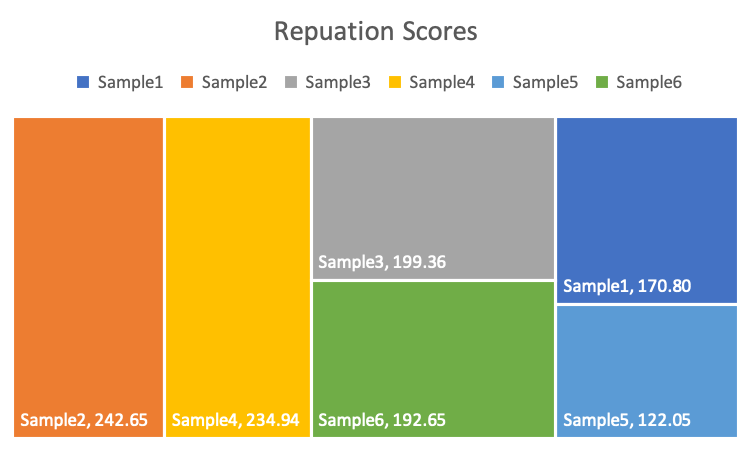
\includegraphics[width=0.7\textwidth]{figures/reputations.png} 
	\caption{The reputations of six samples calculated from July to August 2015}
	\label{reputations} %用于文内引用的标签
\end{figure}

As shown in the figure:
\begin{enumerate}
	\item Sample2 and Sample4 belong to the same class, with high product reputation value, which means better sales prospects; 
	\item Sample3 and Sample6 belong to the same class; Sample1 and Sample5 belong to the same class, with low reputation value, which means that the sales prospects are not clear.
	\item  In fact, we found that Sample5's rating is indeed full of 1-star and 2-star, and there are many bad comments in the reviews.
\end{enumerate}

\subsection{Reputation-Time model Based on RBF Regression}
It is helpful for Sunshine Company to adjust its strategy and increase its profit by exploring the changing law of product reputation over time. Inspired by paper\cite{tang2015user}, we can use neural network to fit and predict reputation.

In this paper, we use RBF neural network as the regression fitting of time based reputation, because RBF has a strong nonlinear fitting ability, can map any complex nonlinear relationship, and the learning rules are simple, which is convenient for computer implementation. The establishment process of our RBF based reputation time model is as follows:
\begin{enumerate}
	\item We first filter the data and select the most representative samples of each type of product:
	\begin{itemize}
		\item \textbf{Pacifier: }'philips avent bpa free soothie pacifier, 0-3 months, 2 pack, packaging may vary' with 833 reviews on 557 dates.
		\item \textbf{Hair Dryer: }'remington ac2015 t|studio salon collection pearl ceramic hair dryer, deep purple', with 587 reviews on 436 dates.
		\item \textbf{Microwave: }'danby 0.7 cu.ft. countertop microwave' with 394 reviews on 224 dates.
	\end{itemize}
	\item By substituting the selected samples into the reputation model, we get the discrete sequence of sample reputation changing with time.
	\item Building RBF network:
	\begin{enumerate}
		\item Take the first half of the sample as the training set and the second half as the test set, then normalize them.
		\item Set the number of neurons in the network to increase gradually, the most is the number of training samples, and set the spread speed to 0.1, start training.
		\item The RBF network was tested and the fitting result was obtained.
	\end{enumerate}
\end{enumerate}
\begin{figure}[H]
\begin{minipage}[t]{0.48\linewidth}	
\centering
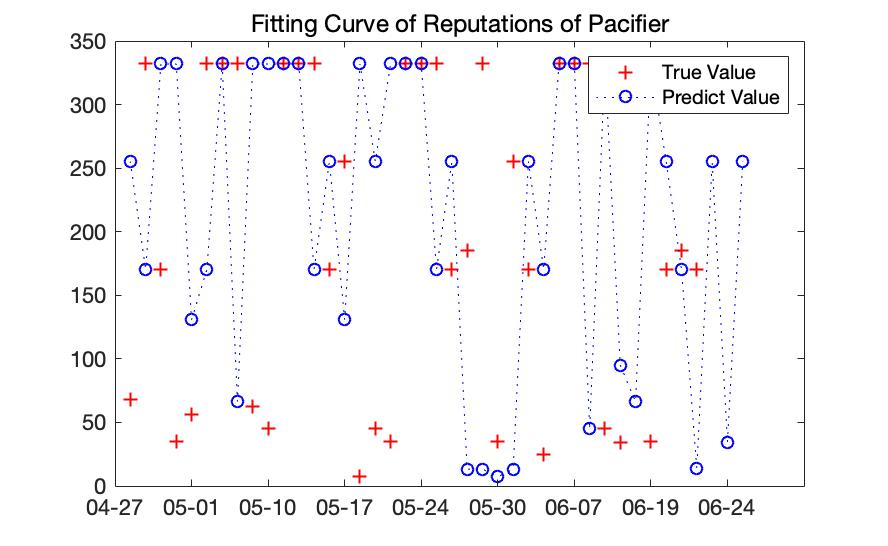
\includegraphics[width=1.0\textwidth]{figures/curve_pacifier.jpg}
\caption{Fitting Curve of Reputations of Pacifier}	  
\label{curve_pacifier}
\end{minipage}
\hfill
\begin{minipage}[t]{0.48\linewidth}	
\centering
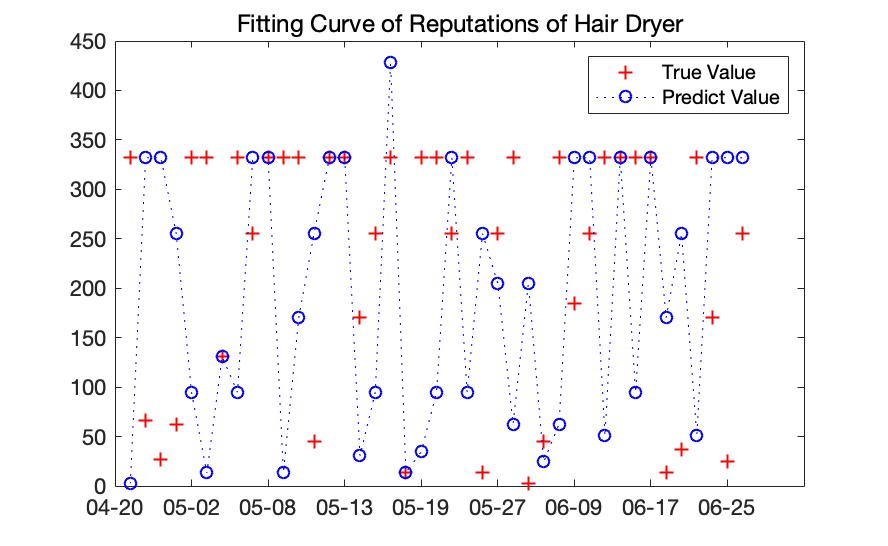
\includegraphics[width=1.0\textwidth]{figures/curve_hair.jpg}
\caption{Fitting Curve of Reputations of Hair Dryer}	  
\end{minipage}
\end{figure}
\begin{figure}[H]
\centering
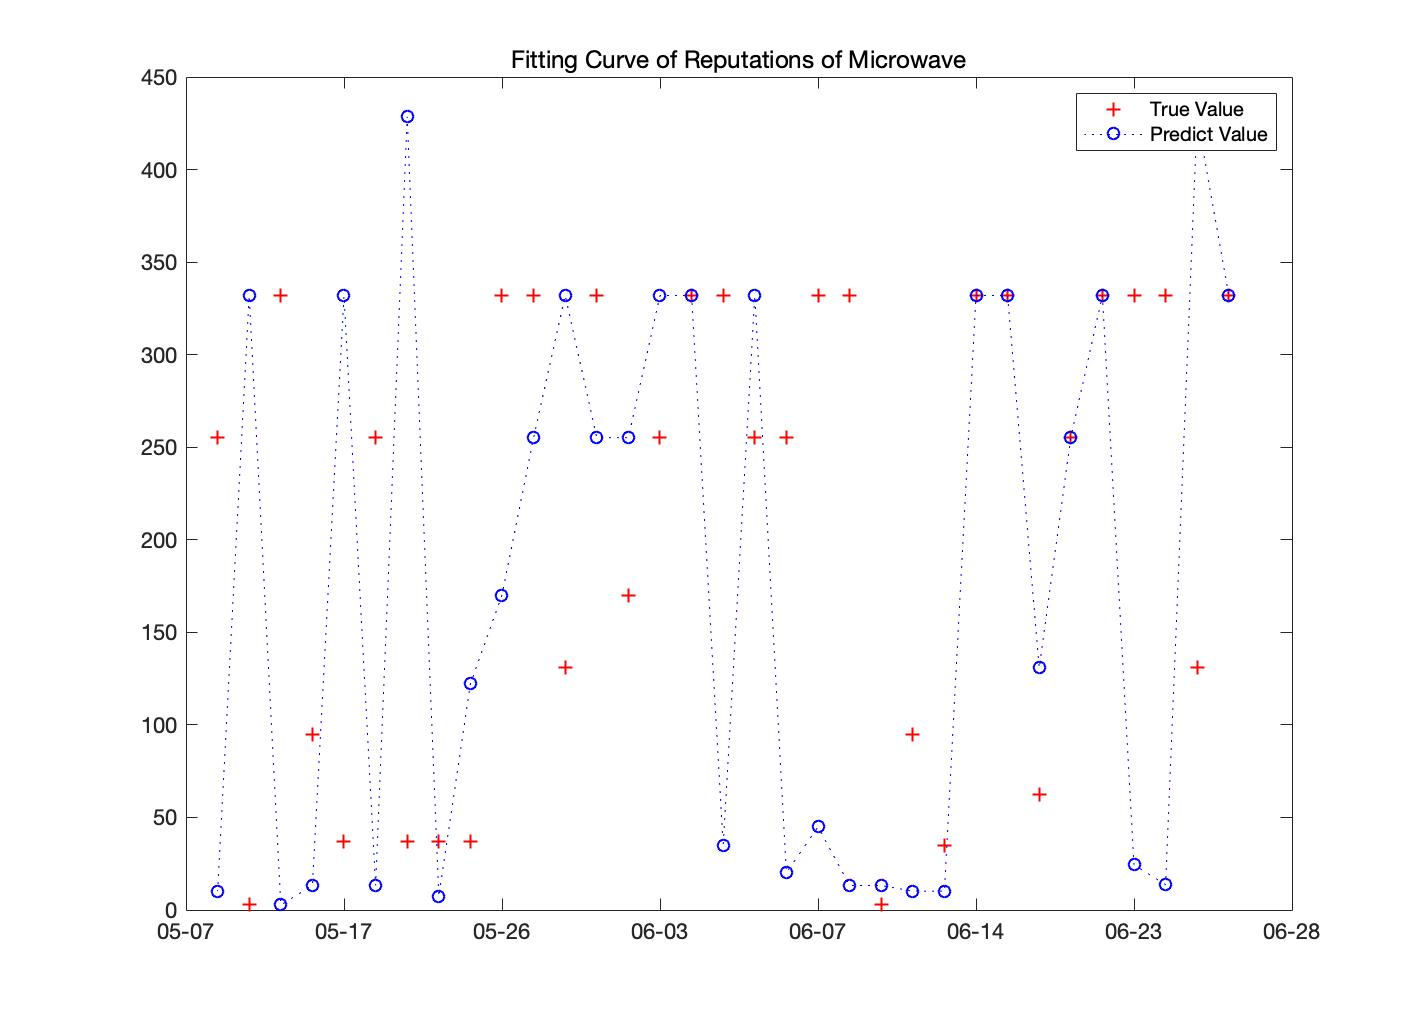
\includegraphics[width=0.48\textwidth]{figures/curve_wave.jpg}
\caption{Fitting Curve of Reputations of Microwave}	  
\end{figure}
From the figure, we can observe the following phenomena:
\begin{itemize}
	\item For pacifier, the minimum reputation appears around May 30, 2015, for hair dryer the minimum appears around May 19, 2015 and microwave's minimal reputation was around June 7. The causes for the minimum will be explained in the next question. 
	\item For pacifier, the maximum reputation value appears around May 10, 2015, for hair dryer the maximum appears around June 9, 2015 and microwave's maximal reputation was around May 26. Again, we will discuss the causes for the maximum in the next question.
\end{itemize}

\subsection{Model to Indicate Potentially Successful or Failing product}
In our modeling, the theme words and ratings near the maximum value of fitting curve are the signs of potential successful products, while the theme words and ratings near the minimum value of fitting curve are the signs of potential failed products.

Take pacifier for example, according to the Fig.\ref{curve_pacifier}, The maximum value of fitting curve appears on May 10, 2015 (marked as $t_{1}$), The minimum value of fitting curve occurs on May 30, 2015 (marked as $t_{2}$), we extract stars and reviews at $t_{1}$ and $t_{2}$'s 7 nearby time points respectively, We conduct LDA text analysis and clustering, and the results are as follows:
\begin{figure}[H]
\begin{minipage}[t]{0.48\linewidth}	
\centering
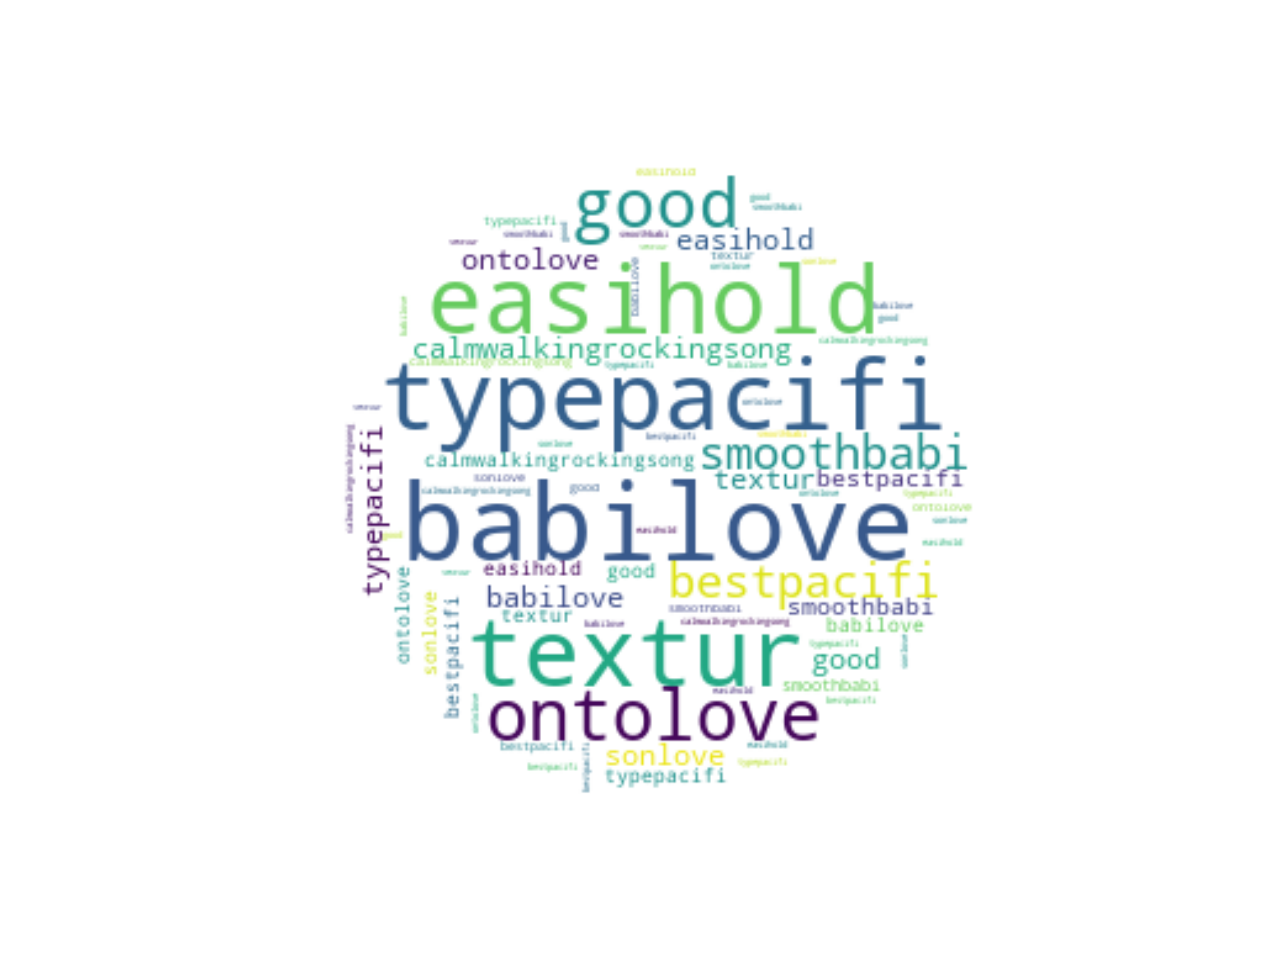
\includegraphics[width=1.0\textwidth]{figures/c_1.png}
\caption{World Cloud for Reviews around May 10, 2015}	  
\label{c_1}
\end{minipage}
\hfill
\begin{minipage}[t]{0.48\linewidth}	
\centering
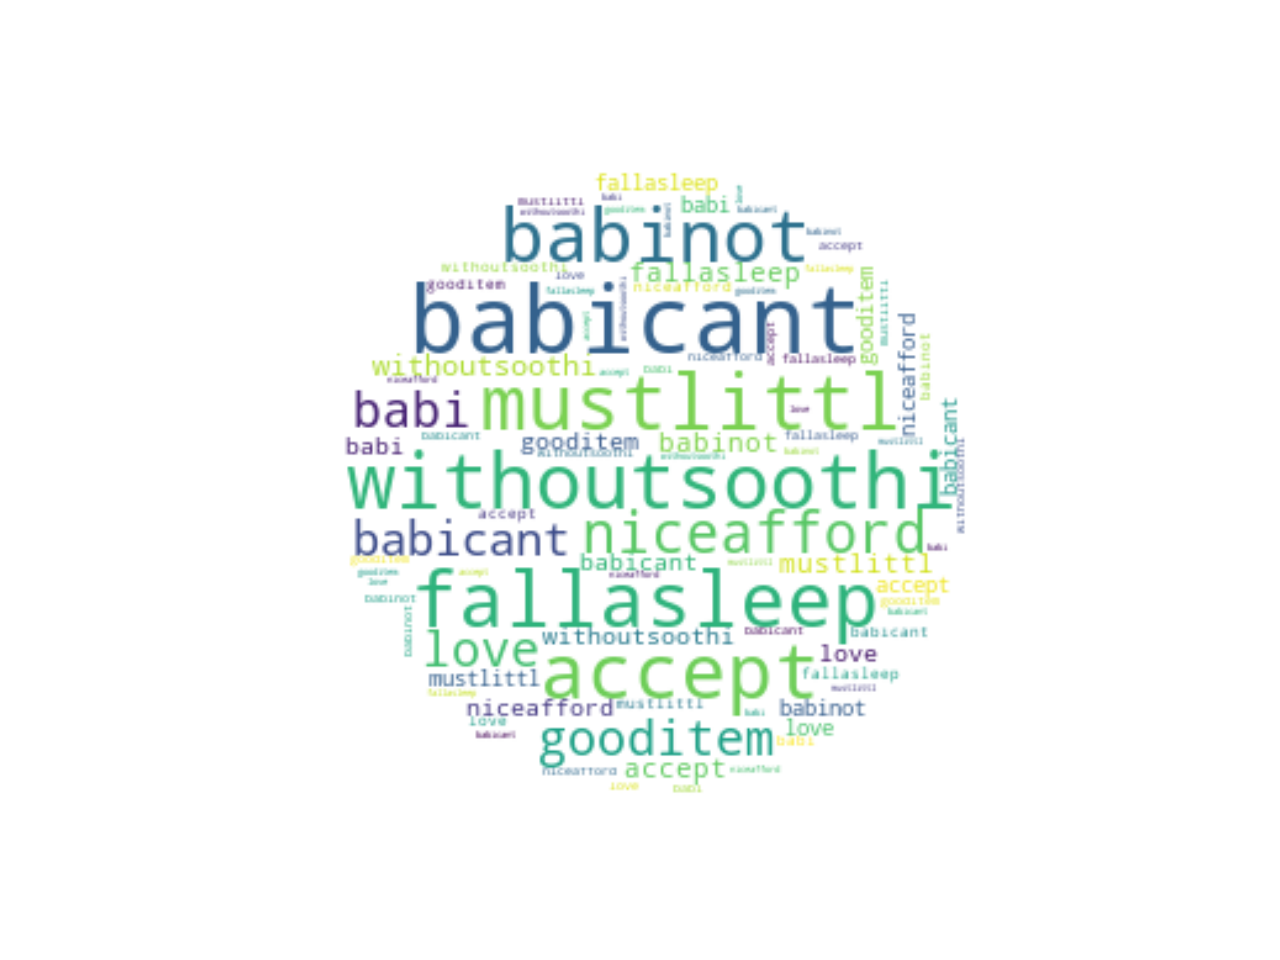
\includegraphics[width=1.0\textwidth]{figures/c_2.png}
\caption{World Cloud for Reviews around May 30, 2015}	  
\end{minipage}
\end{figure}
From the clustering results, we can conclude that:
\begin{itemize}
	\item If the reviews are full of words like 'baby love', 'easy to hold', 'onto love' with 4-5 star ratings, it means that the reputation of the product will usher in a maximum value and it is a potential successful product. So it's recommended for Sunshine Company to grow the portability of pacifiers.
	\item If the reviews are full of words like 'baby cant', 'baby not', 'without soothing' with 2-3 star ratings, it means that the reputation of the product will usher in a minimum value and it is a potential failing product. And we recommend Sunshine Company to fix the soothing problem with the specific pacifier.
\end{itemize}

\section{Sensitivity Analysis}
\subsection{Hyper-parameter $\beta$}
In our reputation model, the super parameter $\beta$ is set to be related to the relationship coefficient $W_{r}$. And we think e-commerce product reviews are more important than ratings\cite{zhang2006lord}, especially the reviews written after experiencing the product, which can better reflect the customer experience. So $\beta$ in our model increased the weight of reviews.

In fact, we find that our model is robust to $\beta$, i.e. slight fluctuations in $\beta$, will not affect the final result of reputation:

We changed $W_{r}$from 0.61 to 0.2 and 1.2 in Eq.\ref{hyperbeta} respectively, and recalculated the samples in section.\ref{task_b}. The results are as follows:
\begin{figure}[H] 
\begin{minipage}[t]{0.48\linewidth}	
	\centering 
	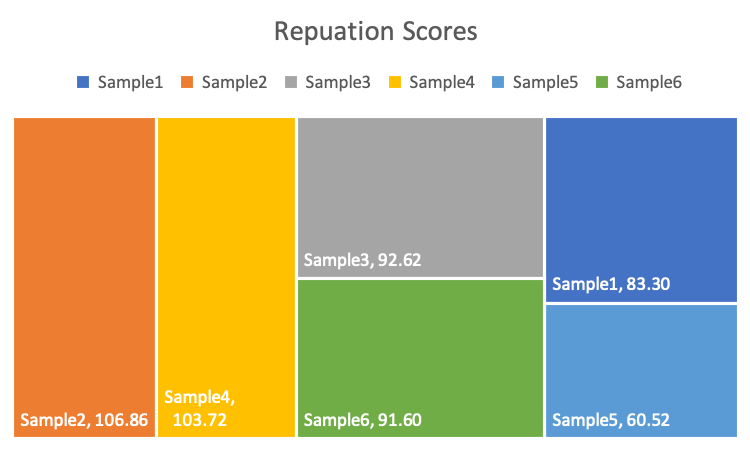
\includegraphics[width=1\textwidth]{figures/reputations_n.png} 
	\caption{The reputations of six samples calculated from July to August 2015 with lower $\beta$}
	\label{reputations_n} %用于文内引用的标签
\end{minipage}
\hfill
\begin{minipage}[t]{0.48\linewidth}	
	\centering 
	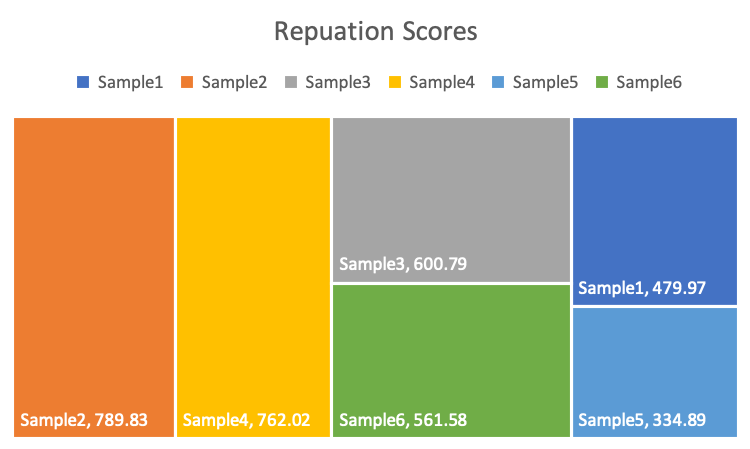
\includegraphics[width=1\textwidth]{figures/reputations_nn.png} 
	\caption{The reputations of six samples calculated from July to August 2015 with higher $\beta$}
	\label{reputations_nn} %用于文内引用的标签
\end{minipage}
\end{figure}

We can see that although the absolute value of reputation has changed, the relative value remained the same. Sample2 and Sample4 are still the first reputable products, and Sample5 is still the product with the worst reputation among the samples.
\section{Strength and weakness}

\subsection{Strengths}
\textbf{Model rationality.} The models we use for reference are all models that have been proved to have strong generalization ability, and our own reputation model also shows certain robustness to hyper-parameters.

\textbf{Reasonable results.} We analyzed the results and found that our results are reasonable and scientific.

\textbf{Make good use of given data.} We eliminate the redundant information and interference information in the given data, and fully mine the potential data wealth in the remaining information.

\subsection{Weaknesses}
\textbf{Lack of sales in given data.} If the sales volume corresponding to the product can be provided in the given data, then our model will be better tested in practice.

\section{Conclusion}

To mitigate the plastic waste problem, we establish a linear programming base model to estimate the environmental impacts of plastic waste, and get the maximal plastic waste amount without further damage to environment. It is proved that the most extent plastic can be reduced to could be confirmed by HSVR model. A minimal target amount of plastic usage is achieved by expending HSVR model. The equity issue can also be solved by dual programming and sensitivity analysis of factors. Finally, we reckon a timeline to approach this realistic minimal target of plastic using amount. 

\newpage


\begin{thebibliography}{99}

%%%
\bibitem{li2016nonlinear}
M.~M. Li and B.~Verma, ``Nonlinear curve fitting to stopping power data using
  rbf neural networks,'' \emph{Expert Systems with Applications}, vol.~45, pp.
  161--171, 2016.
  
  
\bibitem{stoline1981status}
M.~R. Stoline, ``The status of multiple comparisons: simultaneous estimation of
  all pairwise comparisons in one-way anova designs,'' \emph{The American
  Statistician}, vol.~35, no.~3, pp. 134--141, 1981.

\bibitem{tang2015user}
D.~Tang, B.~Qin, T.~Liu, and Y.~Yang, ``User modeling with neural network for
  review rating prediction,'' in \emph{Twenty-Fourth International Joint
  Conference on Artificial Intelligence}, 2015.
  
\bibitem{subkhankulova2006comparative}
T.~Subkhankulova and F.~J. Livesey, ``Comparative evaluation of linear and
  exponential amplification techniques for expression profiling at the
  single-cell level,'' \emph{Genome biology}, vol.~7, no.~3, p. R18, 2006. 

\bibitem{zhang2006lord}
X.~Zhang and C.~Dellarocas, ``The lord of the ratings: is a movie's fate is
  influenced by reviews?'' \emph{ICIS 2006 proceedings}, p. 117, 2006.
  
\bibitem{blei2003latent}
D.~M. Blei, A.~Y. Ng, and M.~I. Jordan, ``Latent dirichlet allocation,''
  \emph{Journal of machine Learning research}, vol.~3, no. Jan, pp. 993--1022.
  
\bibitem{myers2004spearman}
L.~Myers and M.~J. Sirois, ``Spearman correlation coefficients, differences
  between,'' \emph{Encyclopedia of statistical sciences}, vol.~12, 2004.
  
\bibitem{zhang2006lord}
X.~Zhang and C.~Dellarocas, ``The lord of the ratings: is a movie's fate is
  influenced by reviews?'' \emph{ICIS 2006 proceedings}, p. 117, 2006.
\end{thebibliography}

\newpage
%% Generate the Memorandum, if it's needed.
\memoto{Marketing Director of Sunshine Company}
\memofrom{Team 2013573}
\memosubject{A Wealth of Data}
\memodate{March 9, 2020}
%\logo{\LARGE I'm pretending to be a LOGO!}
\begin{memo}[\textbf{Letter to Sunshine Company}]
\noindent Dear Director:

Thank you very much for your trust and hire our team to solve this important problem for you. As we all know, there is a lot of valuable information in the product ratings and reviews. We hope that the information our team digs from the data of pacifier, microwave and hair dryer can help your company to make reasonable sales strategy, and enhance effectiveness of products timely. We hope our suggestions can be helpful to your company. 

%第一问的分析与结果结论,以及意见. 
%
As for how to integrate product ratings and reviews to provide effective information for your company, our team first quantified the text reviews effectively, and then made full use of helpful votes, vine to trace the credibility of the reviews. As the result, a robust model is established. We believe that a good reputation can potentially bring a better sales volume to a product, so we suggest that your company can evaluate the reputation of pacifier, microwave, hair dryer and other products, and then increase the stock of products with high reputation or amplify their publicity. As mentioned in our paper, 'wubbanub infant pacifier - giraffe' is the first choice for online sales of pacifier products from July to August 2015.

Our fitting model uses a powerful RBF neural network to fit the relationship between reputation and time successfully, which can help us better summarize and predict the change of reputation of products. Furthermore we can excavate the potential factors of product success or failure from the maximum and minimum values. As we mentioned in the article, when words like 'baby cant' or 'without soothing' with 2-3 stars appear, we should be extra careful. This is the product the reputation of which  will begin to decline. We recommend your company to improve your products in time according to such signs. When word like 'baby love' or 'easy to hold' with 4-5 stars appears, your company can safely increase the inventory of the product, because the product is about to sell well.

Our statistical model uses one-way ANOVA. After analyzing the average star rating of products in the past period of time and customers' comments of products, we find that when customers see products with lower star rating, they are more willing to publish negative comments; When they see products with higher star rating, they are more willing to publish positive comments. Therefore, we suggest that your company should try its best to improve the products before launching the products, so as to avoid more bad comments caused by low star rating, which will lead to a vicious circle.

We also finds that some words in the comments are related to specific star ratings. For example, the reviews with "disappointed" are closely related to the star rating of one star, reviews with "love" and "great" are closely related to the star rating of five stars. Therefore, we suggest that companies should focus on extracting reviews with emotional words, research and analysis, and optimize products in a timely manner.
%第e问的分析与结果结论,以及意见. 

We would be very pleased if our suggestion could be of benefit to your company. Wish the given advice above would contribute to your work! 

\begin{flushright}
	Your sincerely\\
	 Team 2013573
\end{flushright}

\thispagestyle{empty}

\end{memo}

\end{document}
%%
%% This work consists of these files mcmthesis.dtx,
%%                                   figures/ and
%%                                   code/,
%% and the derived files             mcmthesis.cls,
%%                                   mcmthesis-demo.tex,
%%                                   README,
%%                                   LICENSE,
%%                                   mcmthesis.pdf and
%%                                   mcmthesis-demo.pdf.
%%
%% End of file `mcmthesis-demo.tex'.
